%=========================================================================
% (c) 2011, 2012 Josef Lusticky

\section{Clock subsystem}\label{sec:analysis-clock}
Contiki provides basic clock interface particularly for use of timers
with a simple goal - measuring time.
This interface is common for all supported platforms,
but the particular implementation is platform specific.
The definition of the common interface is located in {\it{core/sys/clock.h}} file
and the specific implementations can be found in {\it{clock.c}} file
in {\it{cpu/}} directory of Contiki source code.

The clock interface provides {\it{clock\_init}} call for initialising the hardware clock,
that is automatically called during boot sequence of Contiki.
The {\it{clock\_init}} call sets up
appropriate counter registers and interrupt service routines as described in section~\ref{sec:analysis-clock}.
This call is implemented as a macro for AVR CPUs, which evaluates to a specific setup code for each
different type of AVR CPU during compilation, and is defined in {\it{cpu/avr/dev/clock-avr.h}} file.
The setup code is not common to all AVR CPUs because of differences among them - e.g. there are usually
only three Timer/Counter modules, but AVR ATmega1284P has four Timer/Counter modules~\cite{avr-datasheet}.

On AVR Raven, 8 bit Timer/Counter~2 clocked from asynchronous 32~768~Hz crystal oscillator
is used by default by Contiki clock interface.
This oscillator is independent of any other clock,
can be only used with Timer/Counter~2 and it
enables use of Timer/Counter~2 as a Real Time Counter~\cite{avr-datasheet}.
The Timer/Counter~2 prescale value 8 is used in Contiki on AVR Raven platform,
so that oscillator frequency 32~768~Hz is effectively divided by 8.
The counter register is hence incremented with frequency
$f_{T2} = {\frac{f_{asy}}{prescaler}} = {\frac{32768}{8}} = 4096$~Hz.
Figure~\ref{fig:avr-clock} shows the Timer/Counter~2 clock module.
\begin{figure}
  \centering
  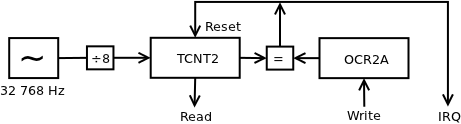
\includegraphics[width=9cm,keepaspectratio]{fig/avr-clock.png}
  \caption{AVR Raven hardware clock}
  \label{fig:avr-clock}
\end{figure}

%%Unlike I/O clock used for clocking other Timers/Counters,
%%this asynchronous crystal is also active in power-save mode~\ref{avr-datasheet}.
%CITATION: If Timer/Counter2 is enabled, it will keep running during sleep. The device can wake up from
%either Timer Overflow or Output Compare event from Timer/Counter2.
%If Timer/Counter2 is not running, Power-down mode is recommended instead of Power-save
%mode.
%The Timer/Counter2 can be clocked both synchronously and asynchronously in Power-save
%mode. If the Timer/Counter2 is not using the asynchronous clock, the Timer/Counter Oscillator is
%stopped during sleep. If the Timer/Counter2 is not using the synchronous clock, the clock source
%is stopped during sleep. Note that even if the synchronous clock is running in Power-save, this
%clock is only available for the Timer/Counter2.

The Timer/Counter~2 module is used in Clear Timer on Compare Match (CTC) mode by Contiki.
In this mode, the counter register {\it{TCNT2}} is incrementing
and the compare register {\it{OCR2A}} defines maximum value for the counter register.
Compare match between counter register and compare register
sets the Output Compare Flag {\it{OCF2A}} and resets the timer to zero~\cite{avr-datasheet}.
This behaviour is illustrated in figure~\ref{fig:design-timing-diagram}
- the {\it{TOP}} value is equal to the value in compare register and the {\it{BOTTOM}} value is equal to zero.

\begin{figure}
  \centering
  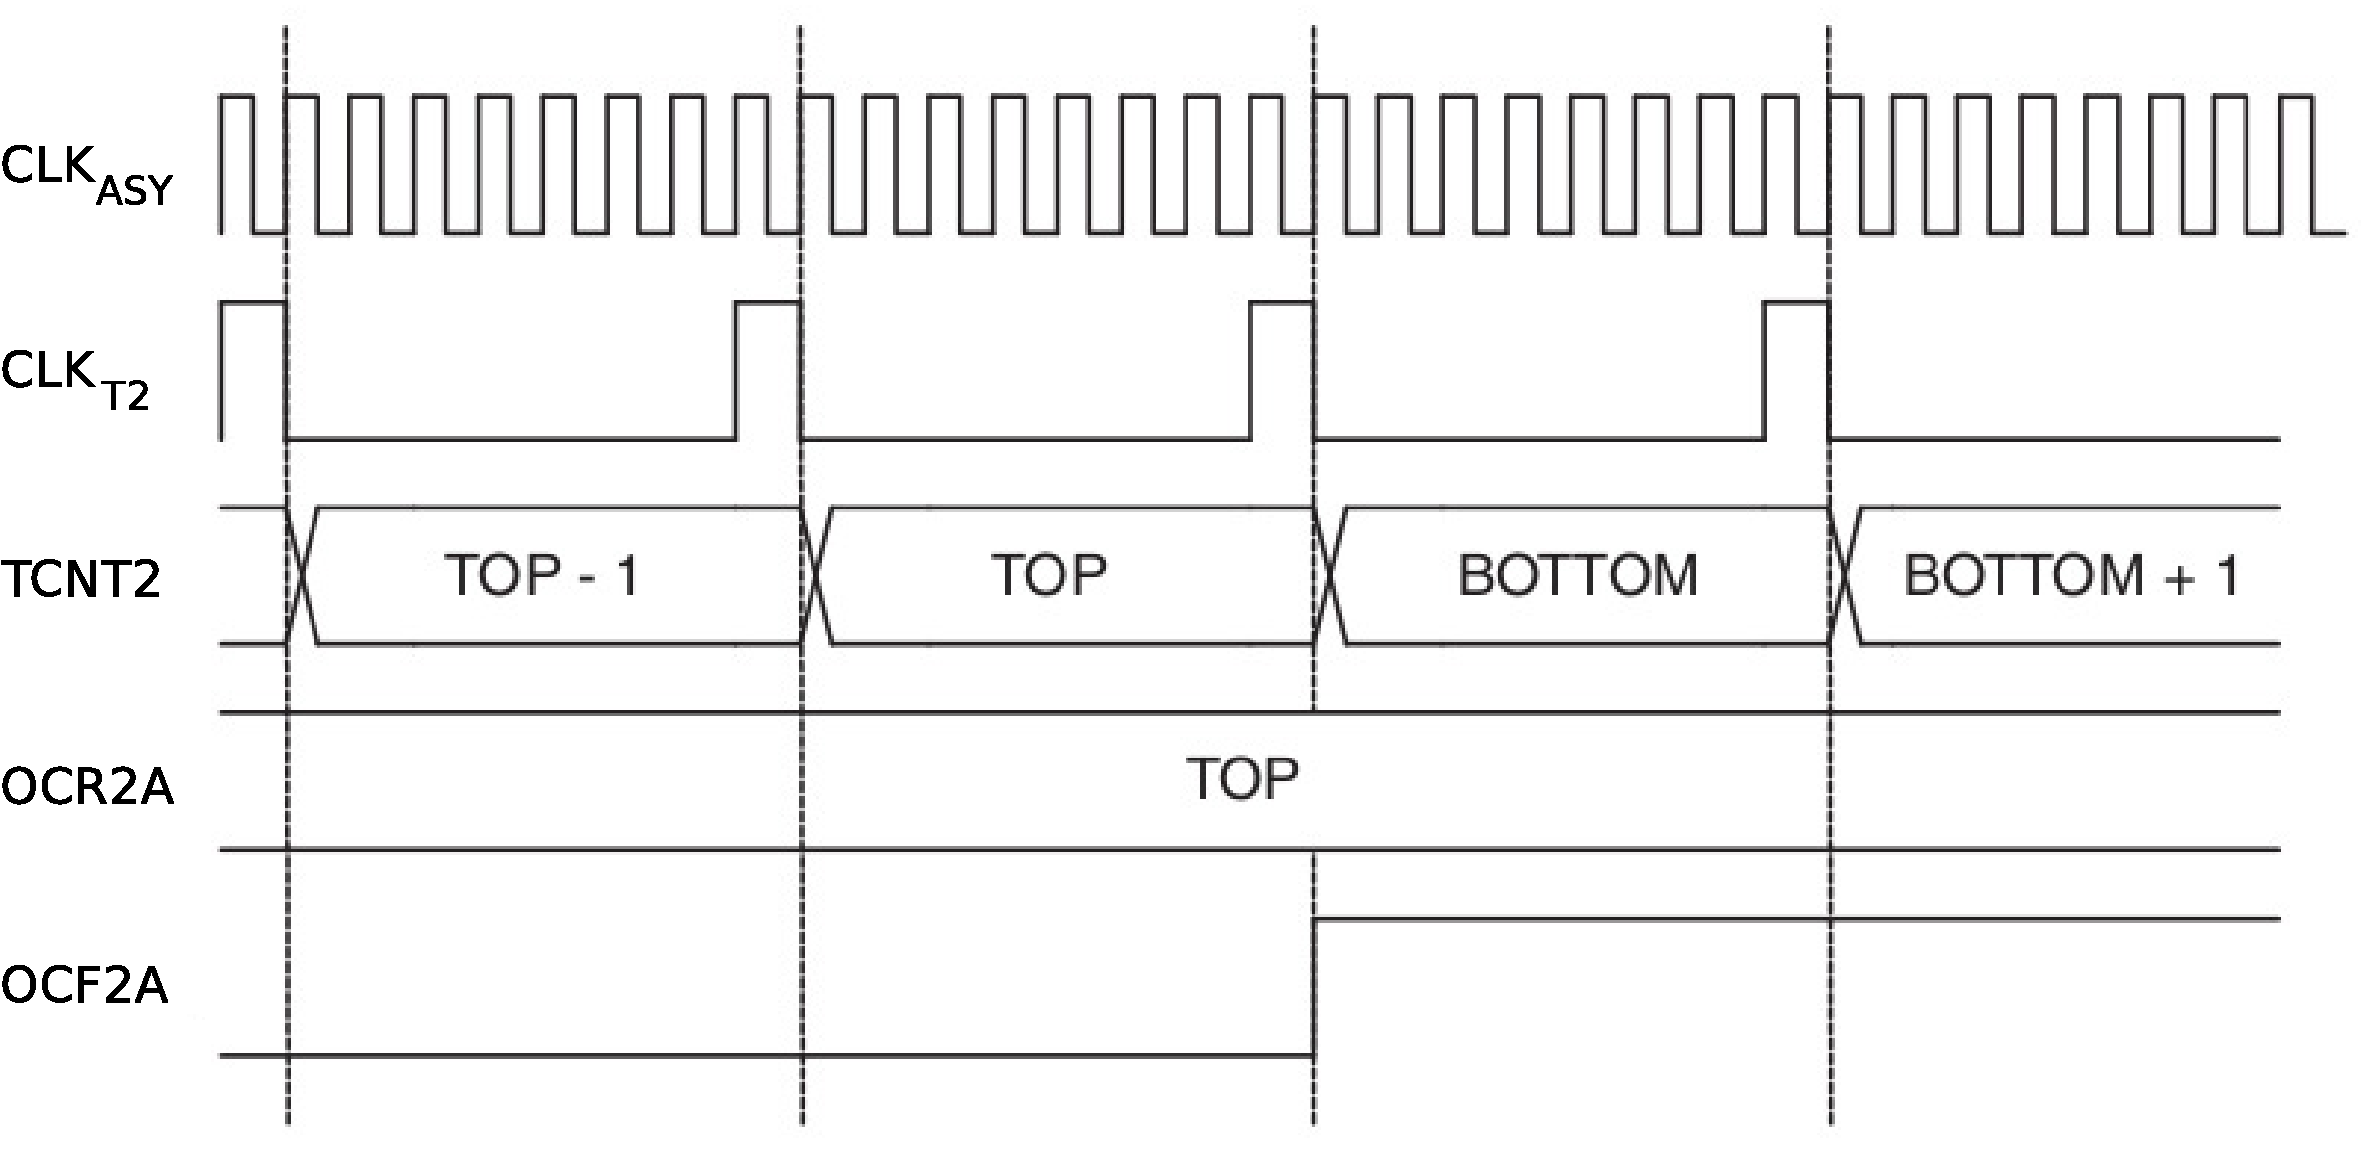
\includegraphics[width=12cm,keepaspectratio]{fig/timing-diagram.pdf}
  \caption{Timing diagram in CTC mode with prescaler 8 (source:~\cite{avr-datasheet})}
  \label{fig:design-timing-diagram}
\end{figure}

Additionally, when compare match occurs,
interrupt is raised and interrupt service routine {\it{AVR\_OUTPUT\_COMPARE\_INT}},
defined in {\it{cpu/avr/dev/clock.c}} file, is executed.
In this case is flag indicating occurred match {\it{OCF2A}}
cleared automatically by hardware when executing
the interrupt service routine~\cite{avr-datasheet}.

To obtain {\it{CLOCK\_SECOND}} interrupts per second, there must be
${\frac{f_{T2}}{CLOCK\_SECOND}}$ hardware clock ticks between two successive interrupts.
On compare match in CTC mode, the timer is reset to zero as
shown in figure~\ref{fig:design-timing-diagram}.
The value zero is also included in the counting - the 0th count of the timer also takes one tick.
Therefore the value of compare register {\it{OCR2A}} must be ${\frac{f_{T2}}{CLOCK\_SECOND}} - 1$
when using Timer/Counter~2 in CTC mode.
The default value of {\it{CLOCK\_SECOND}} for AVR Raven in Contiki is 128,
what implies the default value of compare register ${\frac{4096}{128}} - 1 = 31$.
This value is defined in {\it{platform/avr-raven/contiki-conf.h}} file.

The interrupt service routine can be further used for updating the value in {\it{OCR2A}} compare register.
This can be used for adjusting the time, because decrementing the compare register
value causes a faster increment of the {\it{scount}} variable, which in turn causes
a faster increment of the {\it{seconds}} variable and vice versa.
However, changing {\it{OCR2A}} to a value closer to zero when the counter is running
must be done with care since the CTC mode does not have a double buffering feature.
If the new value written to {\it{OCR2A}} is lower than the current
value of {\it{TCNT2}}, the counter will miss the compare match~\cite{avr-datasheet}.
